\section{Experiments}\label{sec:experiment}
We perform experiments to answer the following questions:
\begin{itemize}
    \item How does ATM compare with state-of-the-art video pre-training and behaviour cloning baselines for learning from action-free videos?
    \item Can ATM be used for learning from video data that are out of the distribution of demonstration data?
\end{itemize}
Our experiments are split into three sections. In Sec.~\ref{sec:video_bc}, we compare ATM with video pre-training baselines on over 130 language-conditioned manipulation tasks in simulation and in the real world. In Sec.~\ref{sec:human_video}, we show that ATM enables effective learning from human videos. Finally, we present ablation results in Sec.~\ref{sec:ablation}.

\begin{figure*}[ht]
    \centering
    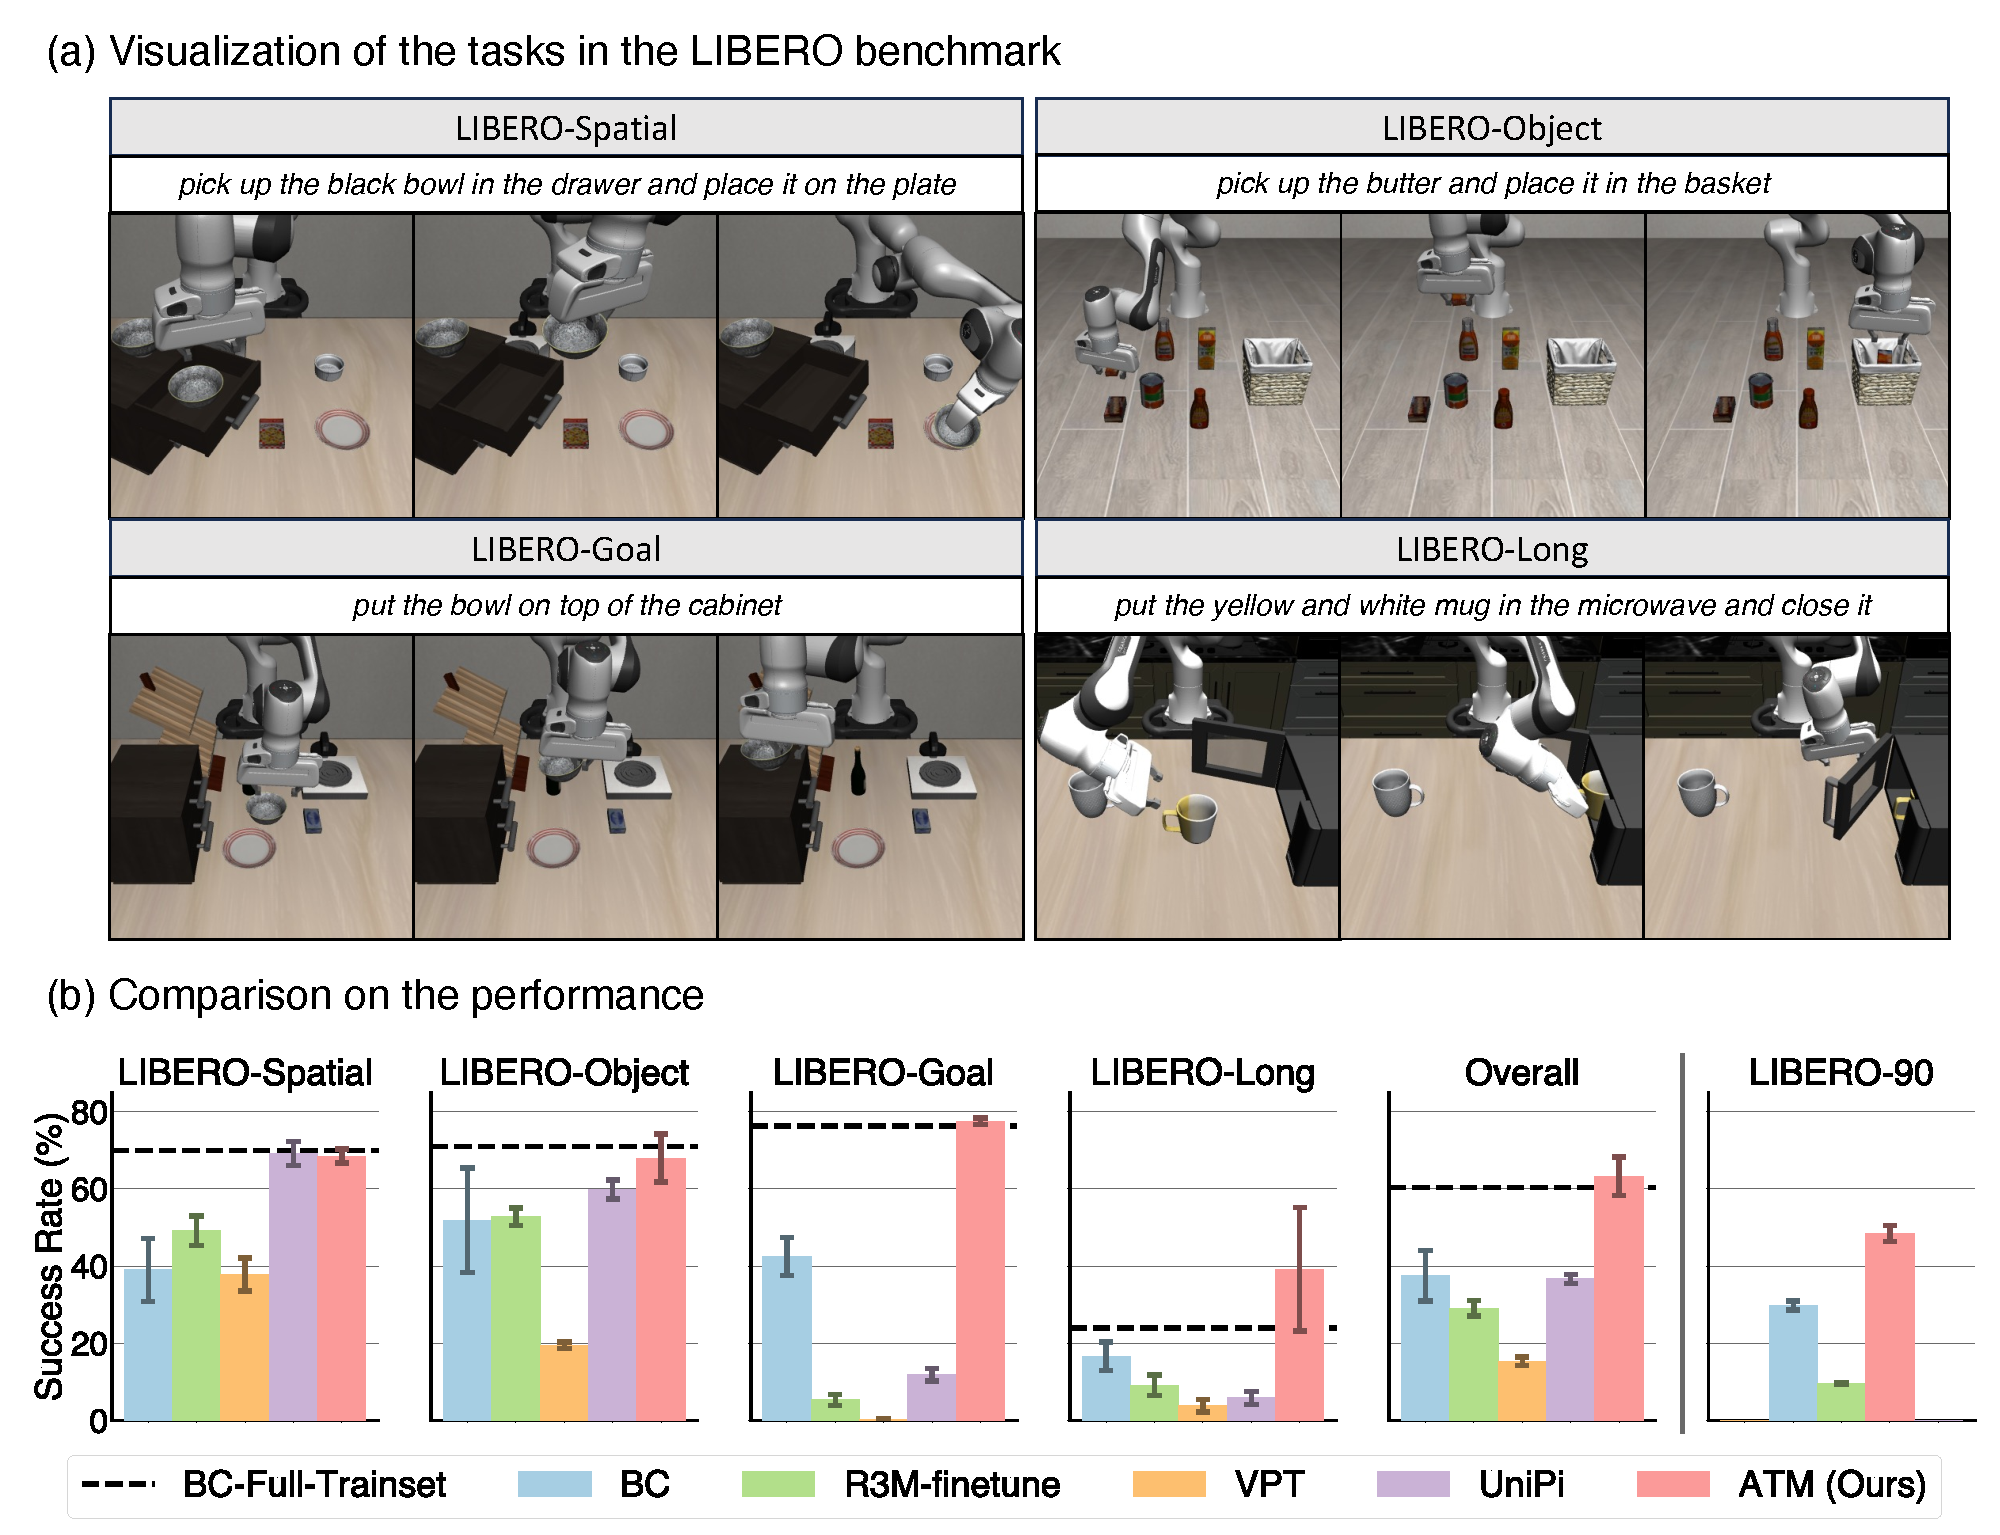
\includegraphics[width=\linewidth]{fig/sim_exp.pdf}
    \caption{We compare with state-of-the-art video pre-training methods on language-conditioned manipulation tasks in the LIBERO benchmark~\cite{liu2023libero}. (a) Visualization of the LIBERO tasks separated into four suites, focusing on different aspects of the manipulation policies in spatial reasoning, object reasoning, task understanding, and performing long-horizon tasks. (b) Quantitative comparisons on different suites. We additionally compare baselines with fast computation on a task suite containing 90 tasks (i.e. LIBERO-90). ATM outperforms the baselines in all tasks and excels in LIBERO-Goal and LIBERO-Long.}
    \label{fig:sim_exp}
\end{figure*}

\begin{figure*}[ht]
    \centering
    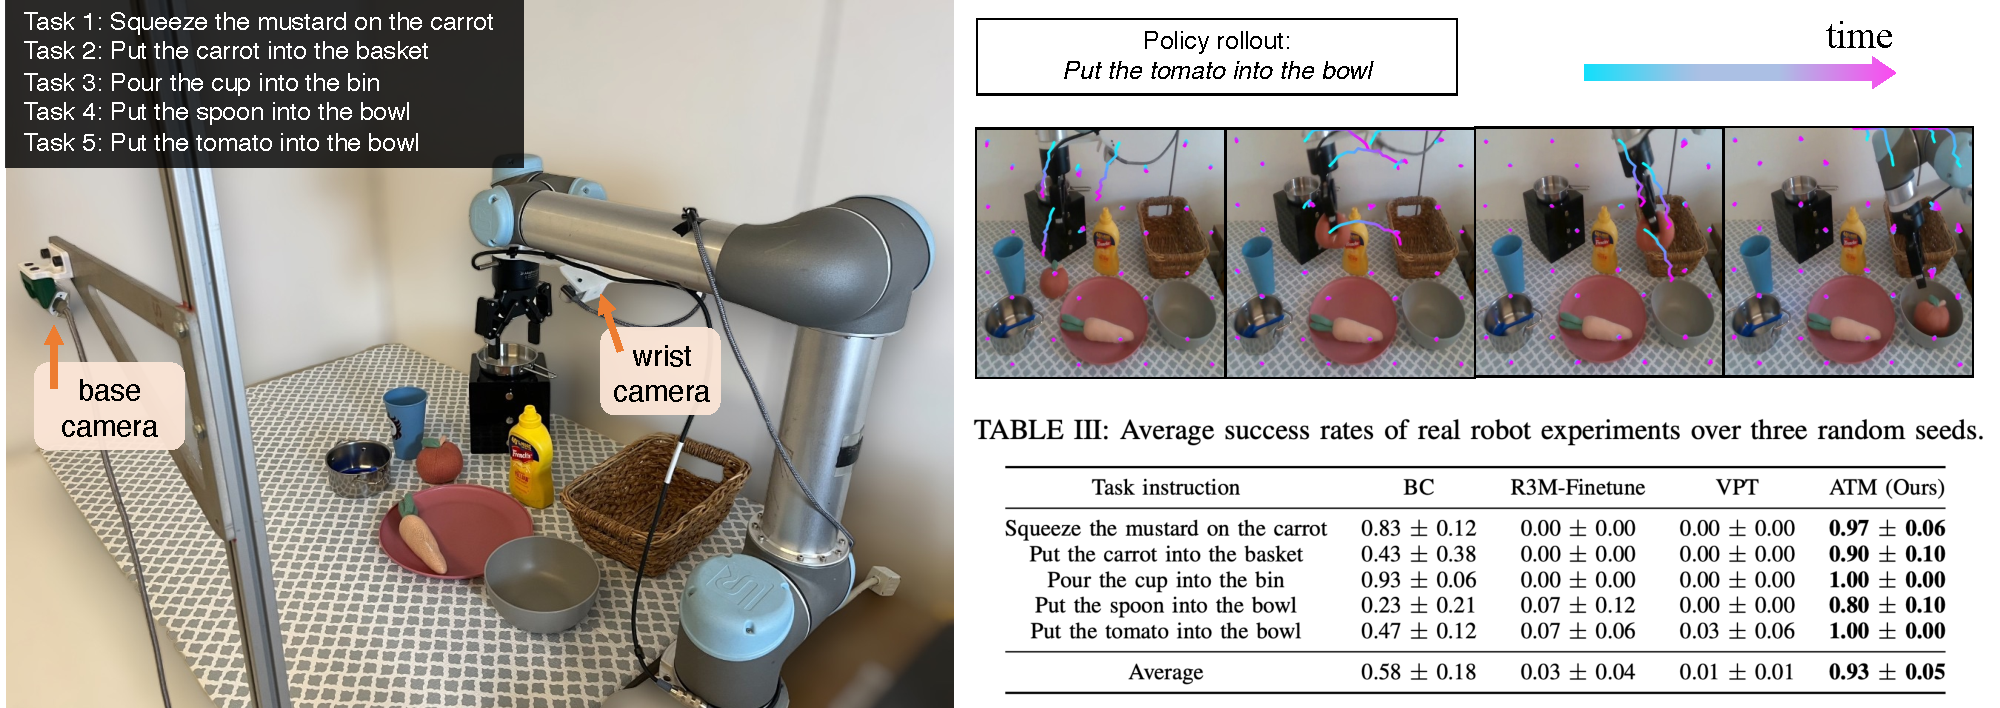
\includegraphics[width=\linewidth]{fig/real_exp.pdf}
    \caption{Real robot experiments on a dining table setup consisting of five tasks. The left figure shows our real-world setup and the tasks. The top right figure shows an example of the predicted particle trajectories and the policy execution, which closely follows the predicted trajectories. From the quantitative results, we can see that ATM shows significant improvements over state-of-the-art video pre-training baselines on average.}
    \label{fig:real_exp}
\end{figure*}

\subsection{Video Pre-training for Imitation Learning}~\label{sec:video_bc}
\noindent\textbf{Environments.} We compare with baselines on over one hundred language-conditioned manipulation tasks in the LIBERO benchmark~\cite{liu2023libero}. The benchmark is subdivided into five suites, LIBERO-Spatial, LIBERO-Object, LIBERO-Goal, LIBERO-Long, and LIBERO-90. Each suite has 10 tasks, except LIBERO-90 which contains 90 tasks. Each task comes with expert human demonstrations. LIBERO-Spatial contains tasks with the same objects but different layouts; LIBERO-Object has tasks with the same layouts but different objects; LIBERO-Goal has tasks with the same object categories and spatial layouts, but different goals; LIBERO-Long has tasks with diverse object categories and layouts, and long-horizon task goals; LIBERO-90 has extremely diverse object categories, layouts and task goals.

\textbf{Data.} We compare with baselines on each suite separately. All methods are trained on $10$ action-labeled demonstration trajectories and $50$ action-free video demonstration trajectories of the robot for each task, amounting to $500$ videos for each 10-task suite. The demonstration dataset contains RGB images from a third-person camera and a wrist camera, together with gripper and joint states as observations. As each task is specified by a language instruction, we use the pre-trained BERT network to obtain a task embedding~\cite{devlin2019-bert}. Image resolution is $128\times128$ and the action space is 7-dimension, representing the translation, rotation, and aperture of the end-effector. 

\textbf{Baselines.}
We compare with the following baselines:
\begin{enumerate}
    \item \textbf{BC} denotes the vanilla behavioral cloning which trains a policy exclusively using the limited action-labeled expert demonstrations, without using the video dataset. It uses a policy architecture identical to ATM except that the particle trajectories are masked to be zero and it instead takes language embedding as task specification. BC baseline can also be considered as an ablation for policy learning without action-free videos. The specific architecture and losses for training the BC policy can vary. We use BC to denote a transformer policy trained using MSE loss by default and compare with diffusion policy separately towards the end of this section.
    \item  \textbf{R3M-finetune}~\cite{nair2023r3m} uses a contrastive learning objective for learning representation that aligns video and language with a combination of time contrastive losses, $L_{1}$ regularization, and language consistency losses. We adopt the publicly released Ego4D pre-trained weights and fine-tune the weights on our in-domain video dataset $\mathcal{T}_o$, to initialize the behavioral cloning policy's visual encoder. During policy training, we also further fine-tune the R3M backbone with the behavioral cloning loss. While this method captures priors from action-free videos through representation learning, the visual representation lacks knowledge about the transition dynamics critical to decision-making.
    \item \textbf{VPT}~\cite{baker2022vpt} first trains an inverse dynamics model from the action-labeled trajectories $\mathcal{T}_a$ and then uses it to predict pseudo action labels for the video dataset. With these pseudo-labels, a policy is then trained with behavioral cloning. This method requires the inverse dynamics model to be robust to a wide distribution of input observation, which can be difficult to learn from the limited demonstrations. 
    \item \textbf{UniPi}~\cite{du2023unipi, Ko2023Learning,black2023zero} trains a text-conditioned video diffusion model to generate a temporally fine-grained video plan from an initial frame and a language instruction. During policy learning, UniPi trains an inverse dynamics model with action-labeled data. We base our implementation off of the UniPi implementation in~\citet{Ko2023Learning}. While both UniPi and ATM leverage a policy conditioned on future subgoals, a trajectory representation decouples motion from other pixel-based information and makes policy learning much easier. Please see the Appendix where we perform additional comprehensive comparisons of different variations of UniPi. 
\end{enumerate}

\textbf{Results.} We present the main results in Figure~\ref{fig:sim_exp}. We see that by bridging the video data and policy learning with the structured representation of point trajectories, ATM~(our method) significantly surpasses various strong baselines in video pre-training, achieving an average success rate of $63\%$ compared to the highest success rate of $37\%$ by previous methods, marking an improvement of over $80\%$. The comparison of BC with ATM shows that learning from additional videos provides useful information for policy learning. VPT performs poorly as we empirically observed that the pseudo-action labels predicted by VPT generally show large errors on the video dataset. UniPi fails on more complex as video prediction models are not physically grounded and often generate future frames that are not physically feasible, such as cases where robots disappear from the image. 
ATM shows surprisingly superior performance on long-horizon tasks and tasks that require an understanding of goals. We attribute this performance gain to ATM's formulation, which utilizes explicit future particle trajectories as subgoals. At each time step, ATM predicts a future trajectory goal based on the current observation. In comparison to the static natural language instructions used by other methods, which do not change throughout the episode, ATM's closed-loop future trajectory provides clear guidance as to what the policy needs to do next.
Please see our video for failure cases of a video prediction model.

\noindent\textbf{Universality of ATM on Different Policy Classes.} The benefit of the predicted trajectories can also be shown for state-of-the-art policy class such as diffusion policy~\cite{Chi2023diffusion}, as shown in Figure~\ref{fig:diff-policy-results}. Here, ATM Diffusion Policy adds the predicted future tracks as additional condition to the policy class, while keeping everything else the same.  We see that ATM consistently improves the performance of diffusion policy across all the suites, achieving the highest scores on the LIBERO benchmark. More details can be found in Appendix.

\begin{figure}[ht]
    \centering
    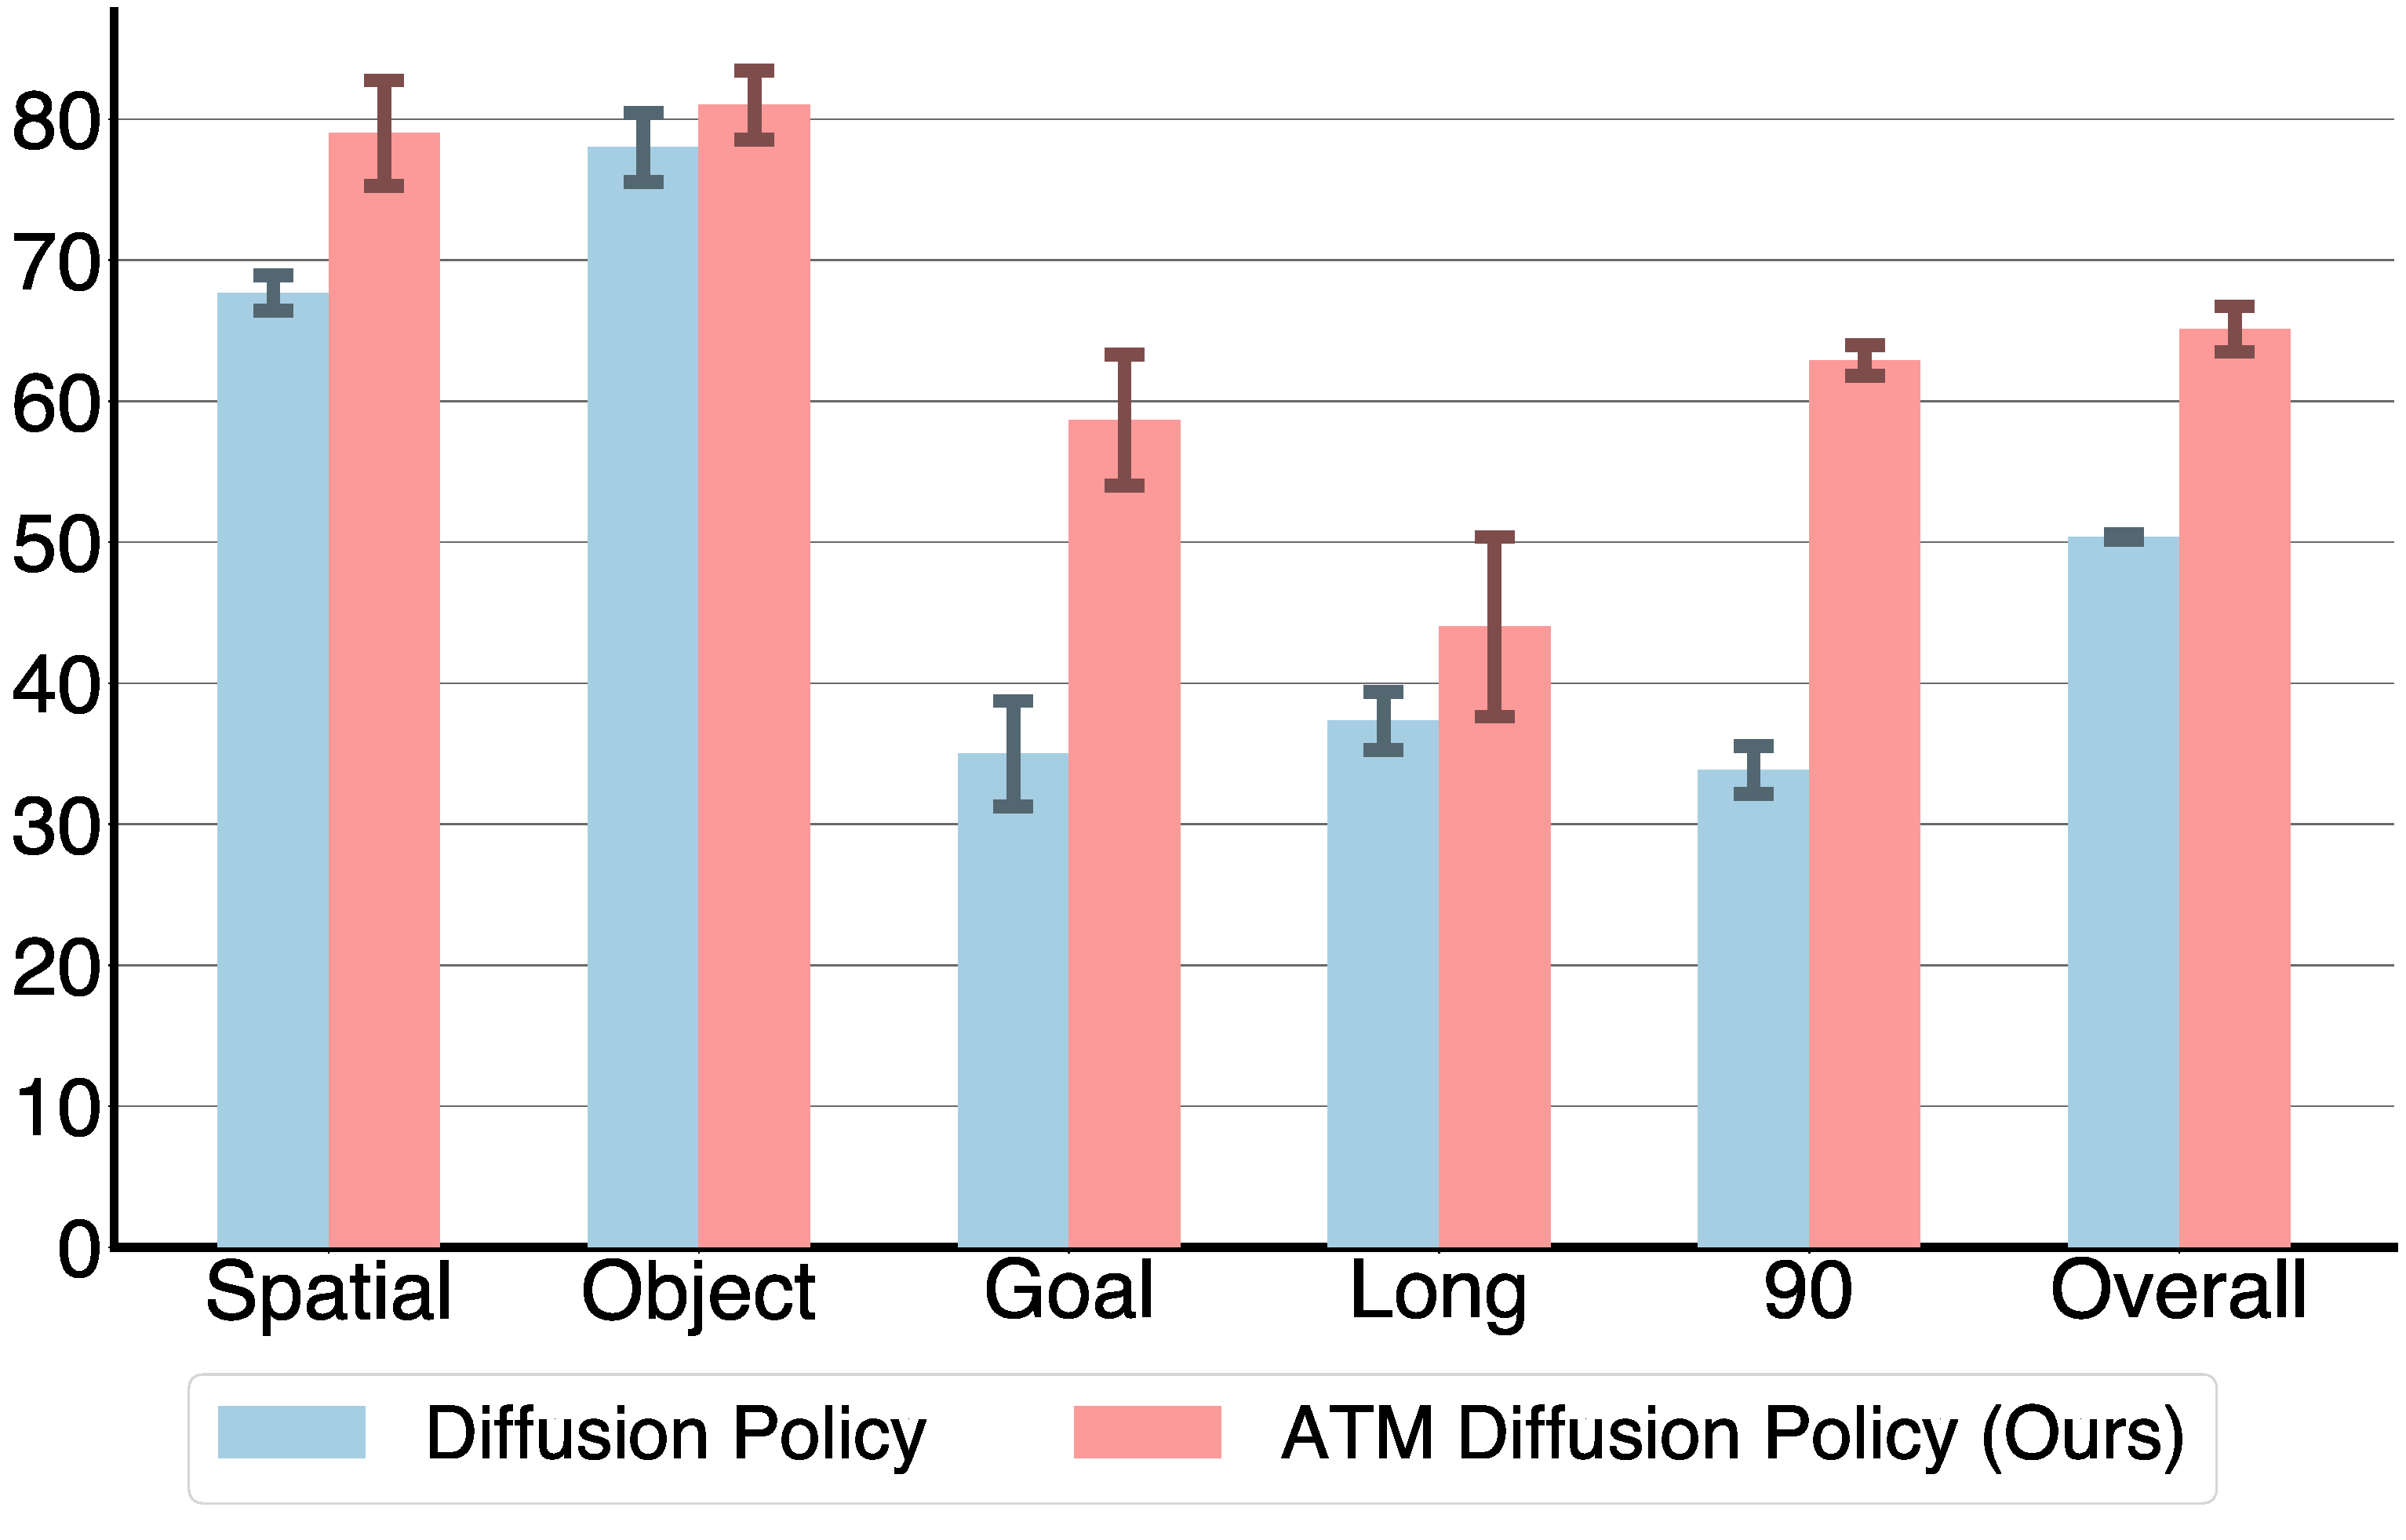
\includegraphics[width=\linewidth]{fig/libero-diffpolicy-success-rate.pdf}
    \caption{We implement ATM Diffusion Policy by adding the predicted future trajectories as additional conditioning and show consistent improvement over the base diffusion policies across the benchmark suites.}
    \label{fig:diff-policy-results}
\end{figure}

\textbf{Real World Setup.} We conduct a language-conditioned manipulation experiment in the real world to further strengthen our claim. As illustrated in Figure~\ref{fig:real_exp}, we learn policies for a 6-DOF UR5 robot arm using human expert demonstrations collected with the GELLO teleoperation system~\cite{wu2023gello}. The action space is joint position control and gripper state. The observations include two RGB images from two RealSense cameras. To compensate for the partial observation, we stack the most recent two frames as the input of agents. We do not feed proprioception states into agents because it is reported that imitation policies tend to overfit them and ignore the visual inputs, leading to worse online rollout performance~\cite{robomimic2021,lin2023spawnnet}. We collect a total of $50$ action-labeled trajectories and $250$ action-free demonstration videos (by simply removing the actions from the collected action-labeled demonstrations). From the quantitative results in Figure~\ref{fig:real_exp}, we see consistent trends that ATM outperforms BC and other video pre-training baselines by a significant margin.

\begin{figure*}[ht]
    \centering
    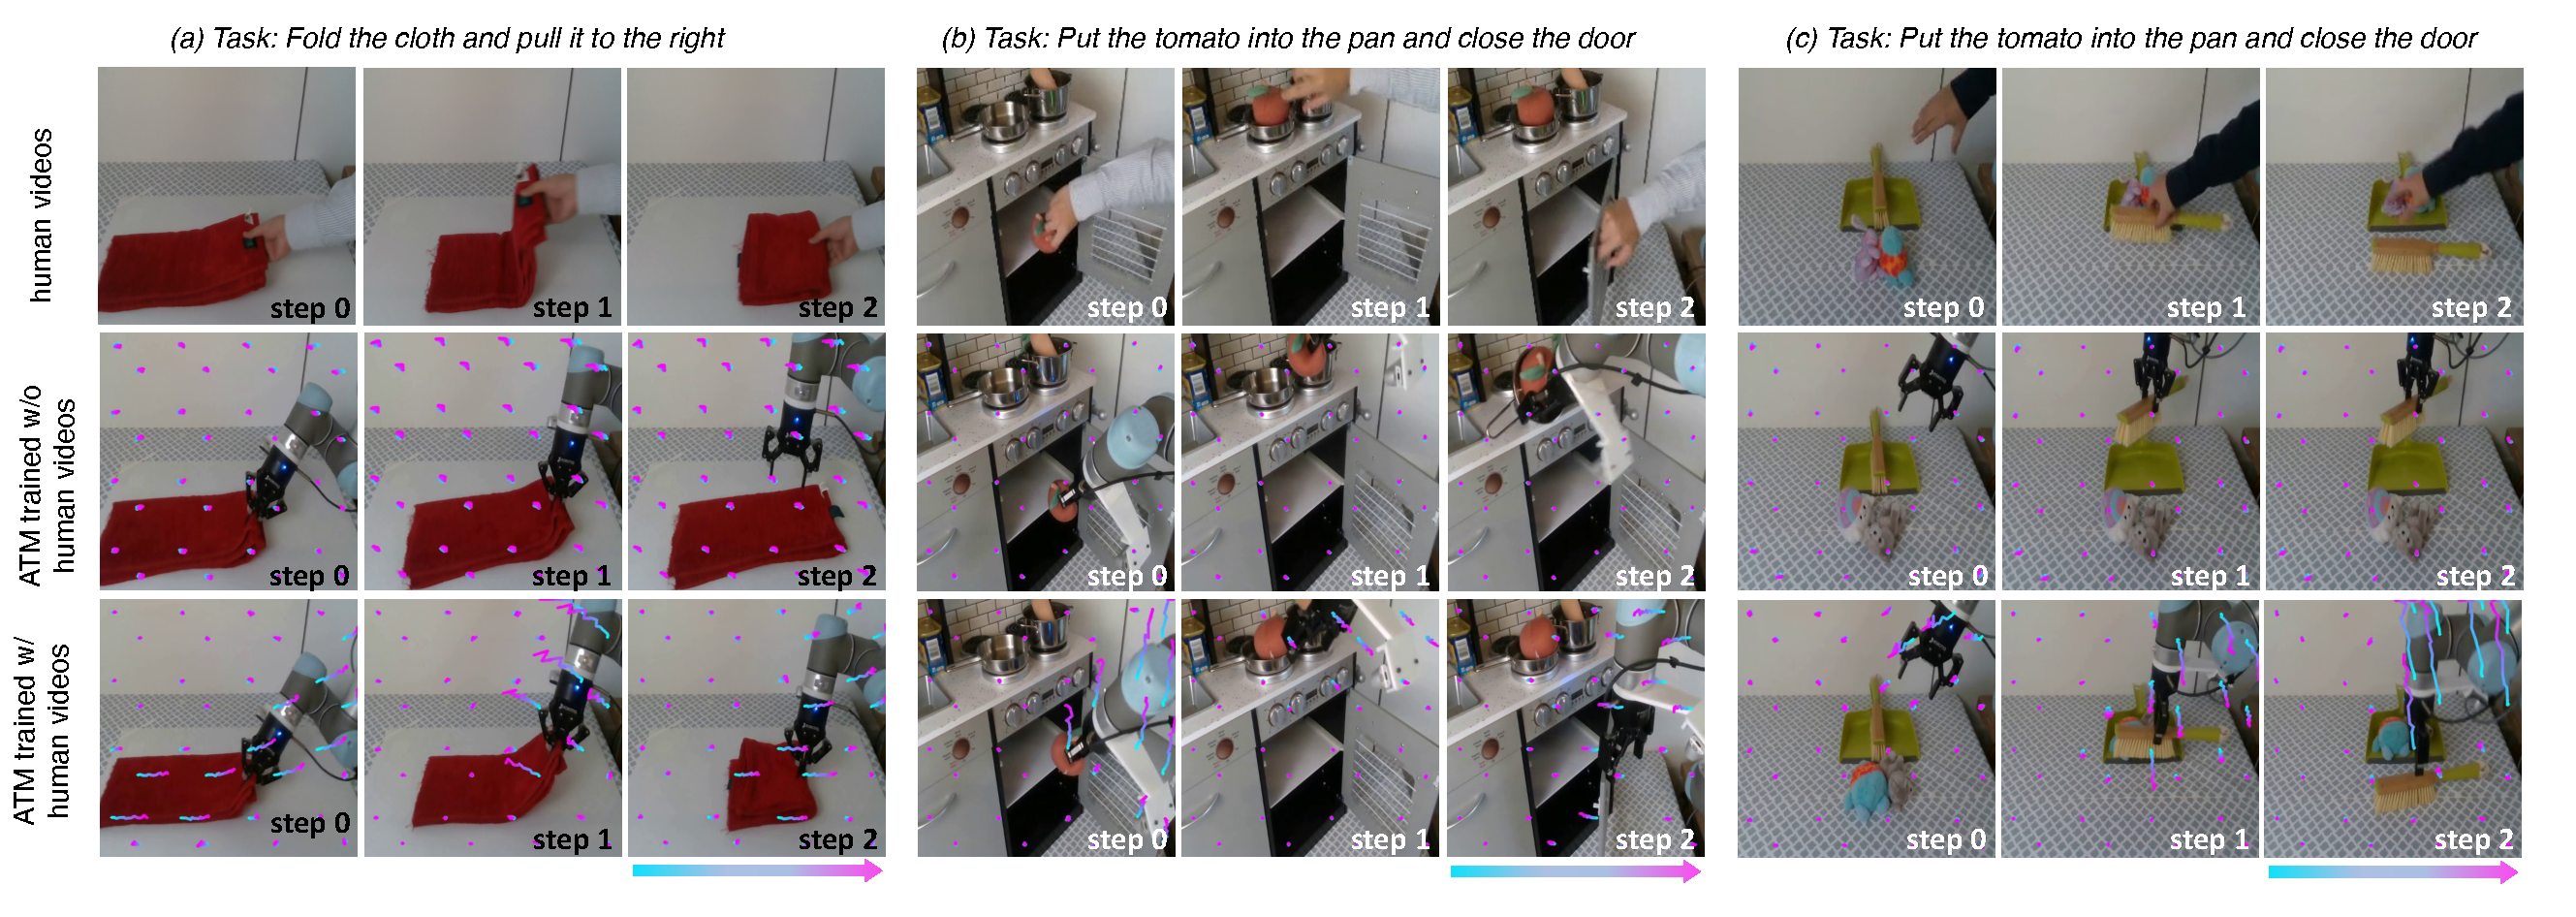
\includegraphics[width=\linewidth]{fig/human_video.pdf}
    \caption{Learning robotic skills from human videos for three tasks. We collect 100 videos of a human performing the tasks directly and 10 teleoperation demonstration trajectories. Each row from the top to the bottom shows three snapshots from the human videos, ATM trained without the human videos, and ATM trained with the human videos. By comparison, we can see that human videos are critical in learning accurate trajectory prediction and enable the policy to successfully perform the task.}
    \label{fig:human_video}
\end{figure*}

\begin{figure*}[ht]
    \centering
    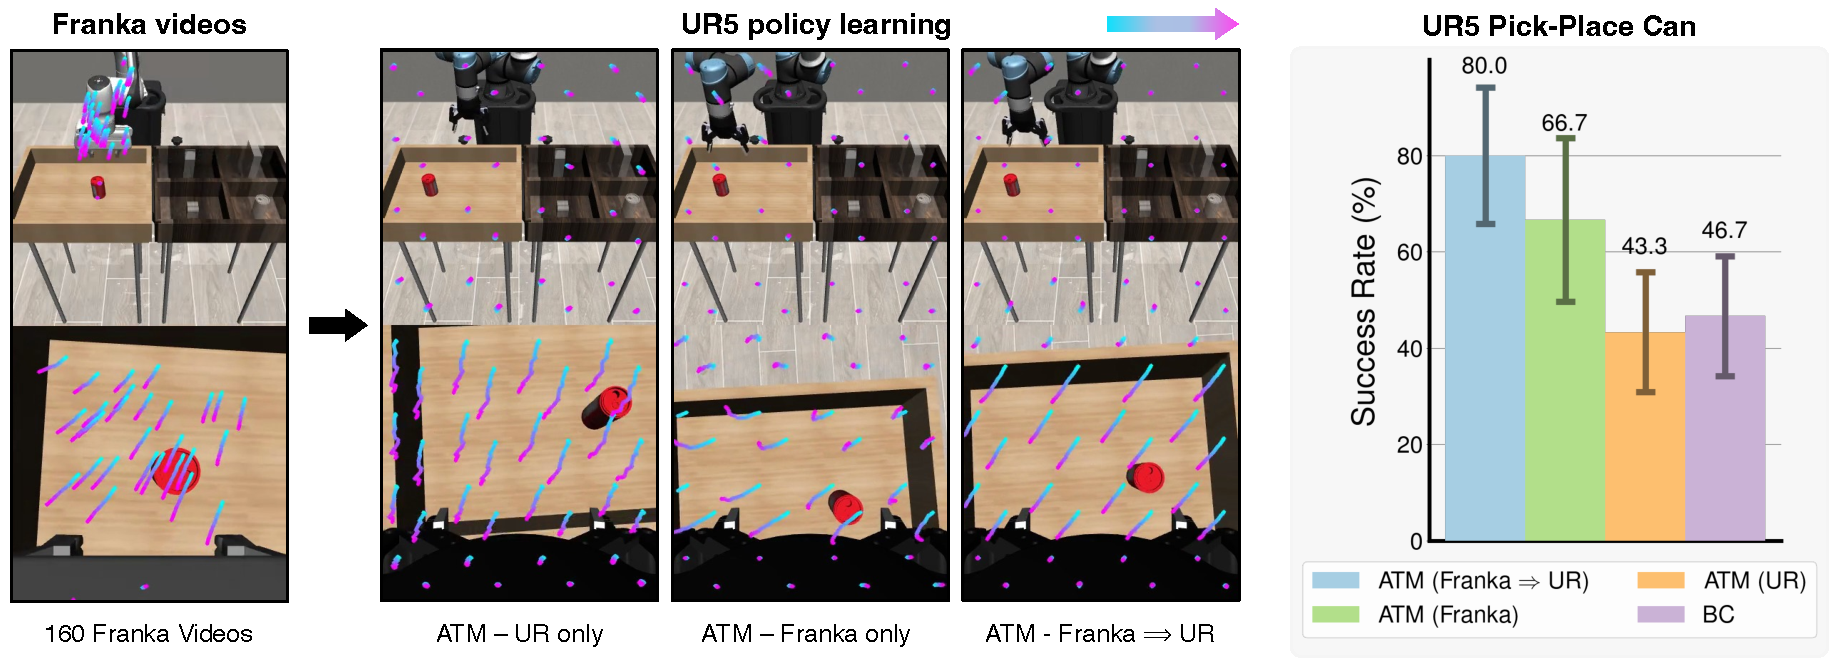
\includegraphics[width=\linewidth]{fig/rob-rob.pdf}
    \caption{Cross-morphology skill transfer for a pick-and-place task. Here, we collect 160 action-free videos of a Franka arm and 10 action-labeled demonstrations from a UR arm, with the final goal of learning a UR policy. We compare a vanilla BC baseline with ATM trained using types of data: using only the 10 UR videos, using only the 160 Franka videos, and using both Franka and UR videos  (Franka $\Rightarrow$ UR). In the right plot, we observe that the additional cross-embodiment data led to significantly better results. Surprisingly, even if the trajectory model is only trained using Franka videos, it exhibits much better performance than the BC without the Franka videos.}
    \label{fig:rob-rob}
\end{figure*}

\begin{table}[ht]
  \centering
  \caption{Average success rates of human-to-robot experiments. ATM trained with human videos significantly outperforms BC and ATM trained with only 10 robot videos, demonstrating the cross-embodiment capability of ATM.}
  \begin{tabular}{@{}cccccc@{}}
    \toprule
     Method & \specialcell{Teleoperation \\ demos} & \specialcell{Human \\ videos} & \textit{fold cloth} & \textit{put tomato} & \textit{sweep toys} \\
    \midrule
    BC & \CheckmarkBold & \XSolidBrush & 0\% & 10\% & 30\% \\
    ATM & \CheckmarkBold & \XSolidBrush & 0\% & 0\% & 13\% \\
    ATM & \CheckmarkBold & \CheckmarkBold & \textbf{63}\% & \textbf{63\%} & \textbf{60\%} \\
    \bottomrule
  \end{tabular}
  \label{tab:human-robot-result}
\end{table}

\subsection{Human-to-robot and Robot-to-robot Transfer} \label{sec:human_video}
By modeling the low-level any-point trajectories, ATM enables learning from cross-embodiment videos of humans or a different robot performing the task. This facilitates the use of more scalable data sources. To verify this, we present the results of learning from human videos in Fig.~\ref{fig:human_video}, with the quantitative results presented in Table~\ref{tab:human-robot-result}, and the results of cross-robot transfer in Fig.~\ref{fig:rob-rob}. We compare the following methods: \textit{(1)} Learning behavior cloning policies only on the action-labeled data \textit{(2)} ATM, using a track transformer trained only on the limited action-labeled robot data, and (3) ATM, using a track transformer trained on both the action-free human and action-labeled robot data. Experiments show that training the trajectory model on additional cross-embodiment videos makes the trajectory prediction more robust and accurate, significantly improving policy learning. On the other hand, as the number of action-labeled trajectories is small, BC baselines that only use action-labeled trajectories fail. Please refer to the videos on our website for better visualization. 


\subsection{Ablation Analysis} \label{sec:ablation}
We conduct a series of ablation experiments in simulation to demonstrate the effect of our design choices. These include the number of action-labeled trajectories needed for policy learning, the effect of the trajectory prediction horizon, image masking, and late track fusion. Besides, we also investigate the universality of ATM for different policy models.

\begin{figure}[ht]
    \centering
    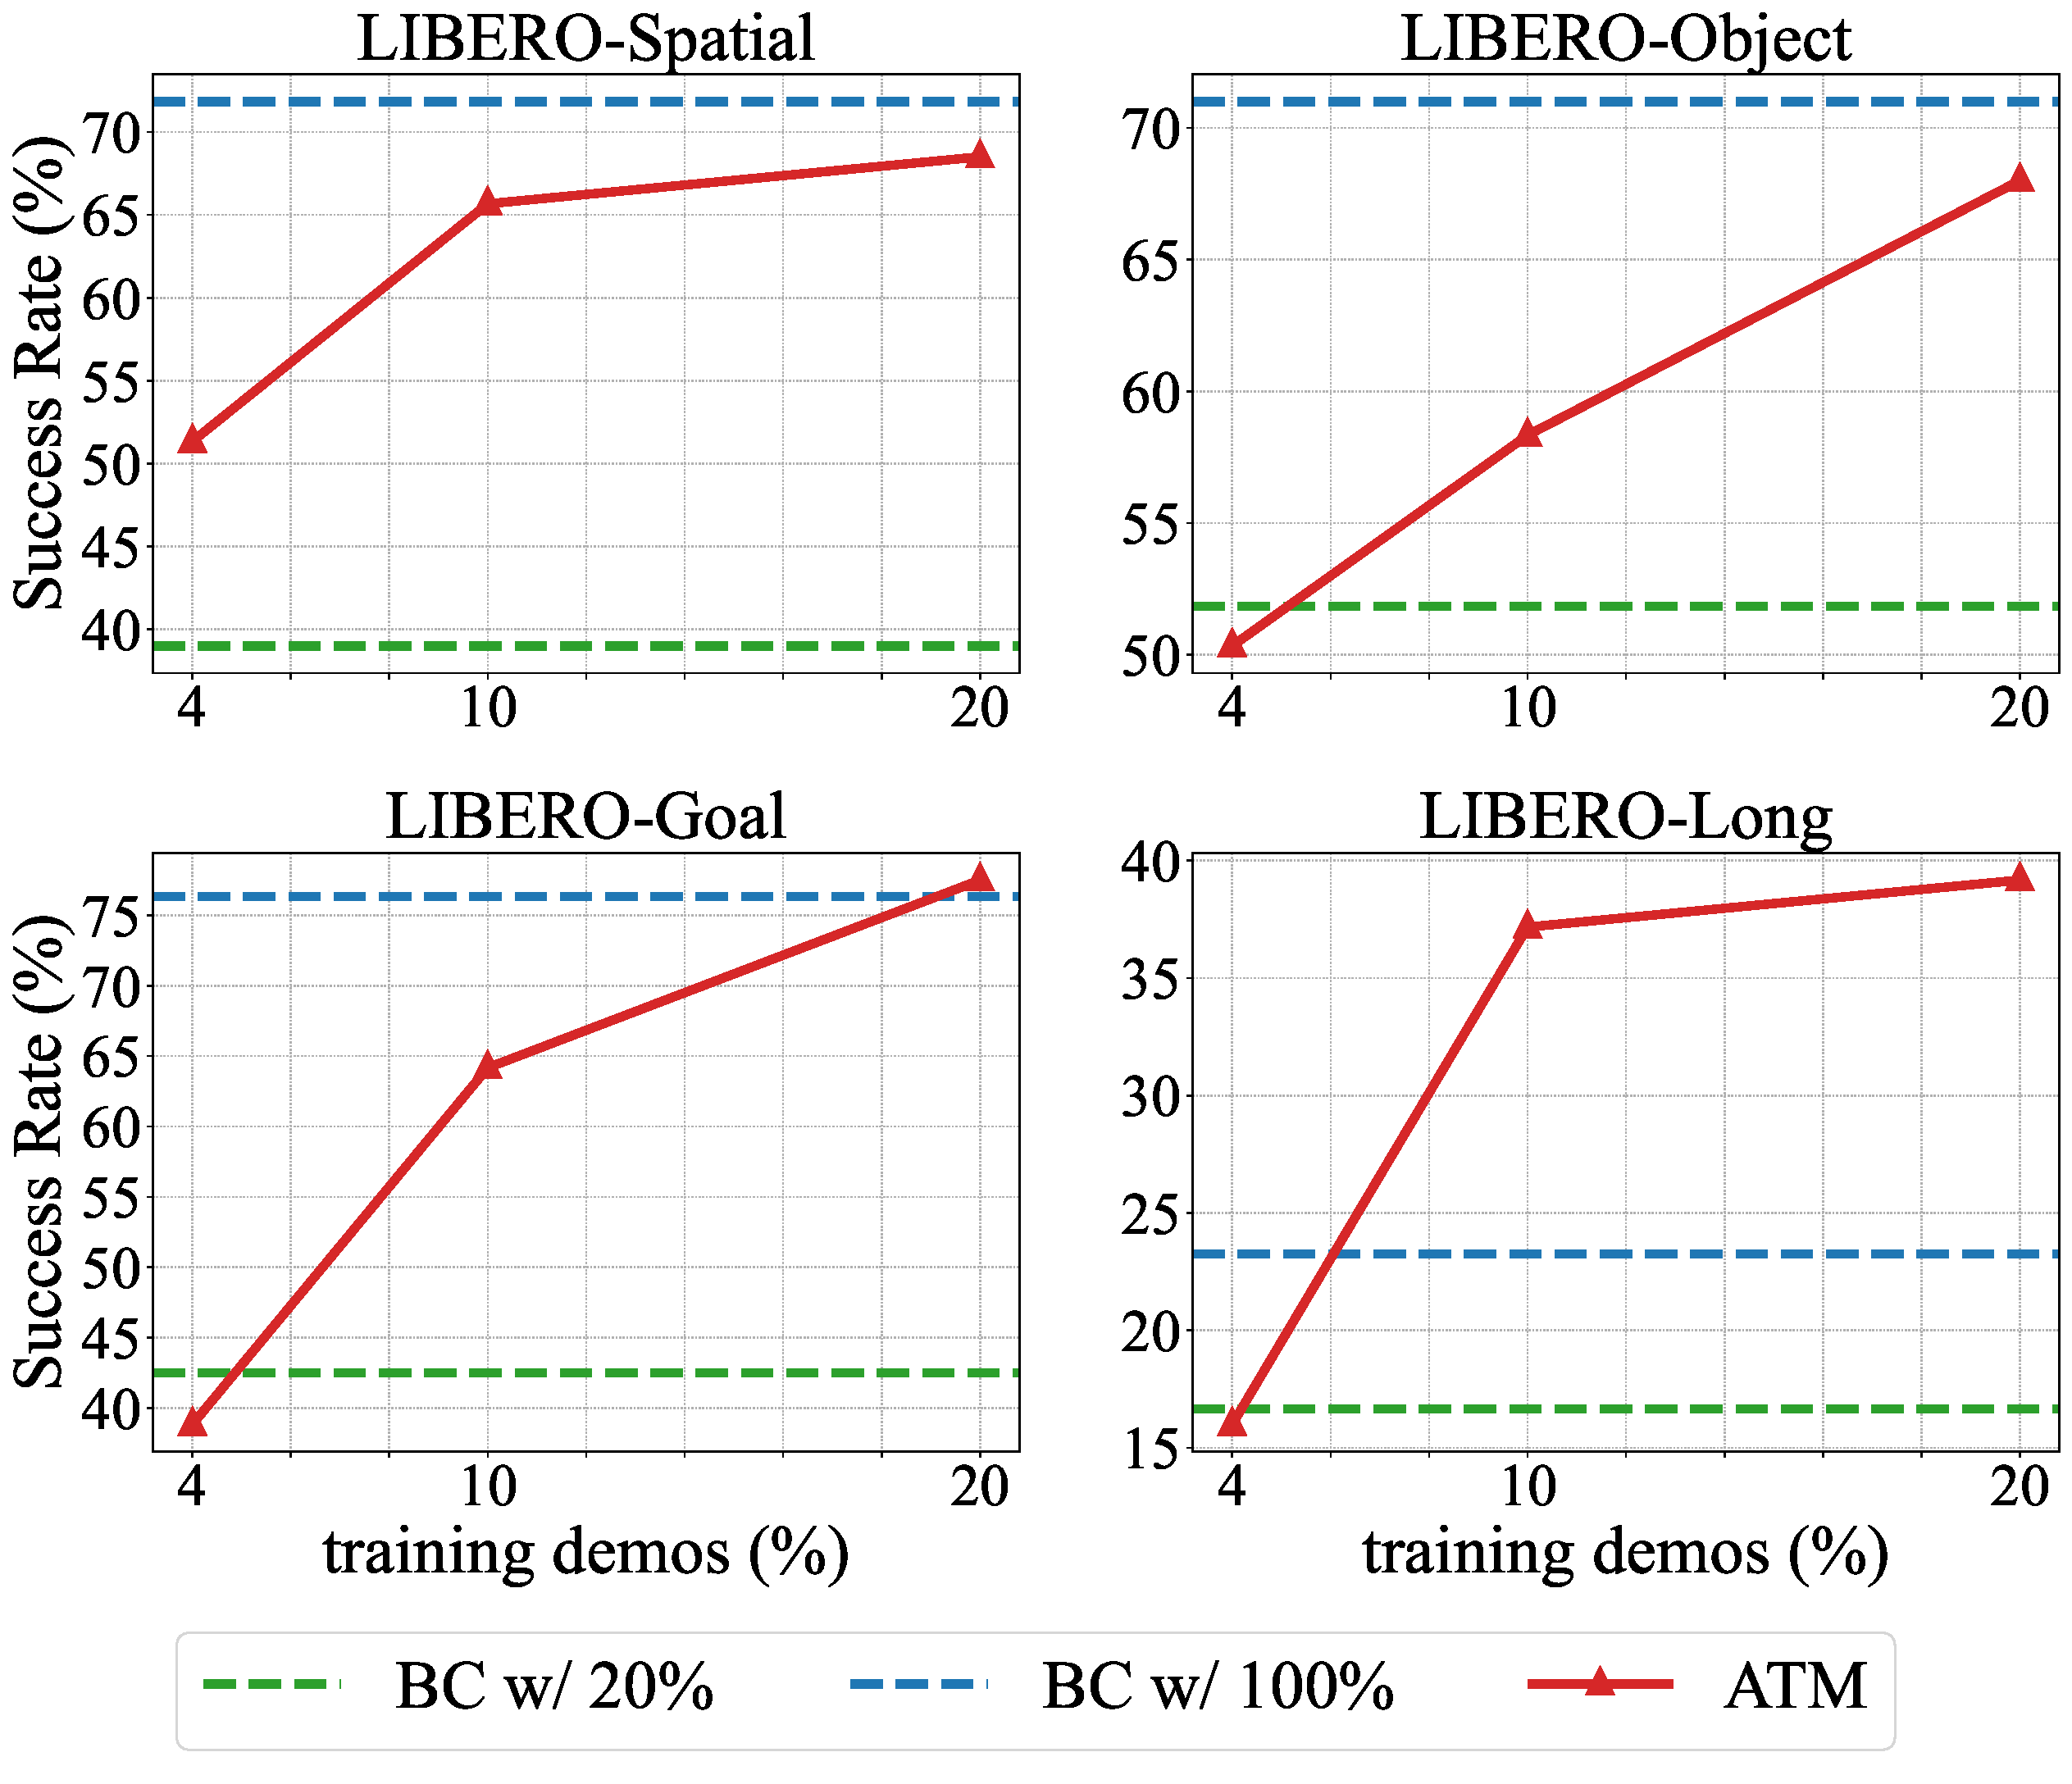
\includegraphics[width=\linewidth]{fig/libero-num-demos-with-bound.pdf}
    \caption{Success rate of our policy trained with 4\%, 10\% and 20\% action-labeled demos. Our policy trained with only 4\% demos performs comparably to BC baseline with 20\% demos on LIBERO-Spatial, Object, and GOAL, and even better on LIBERO-Spatial. When trained on 20\% demos, our performance approaches BC with all training data.}
    \label{fig:num-demos}
\end{figure}


\noindent\textbf{Effect of the number of action-labeled trajectories.}
We investigate the impact of track length on our policy input by training our policy using predicted tracks of varying lengths: 4, 8, 16, 32, and 64 steps.
As illustrated in Figure~\ref{fig:libero-track-len}, a track length of 16 yields optimal performance on average. Smaller track lengths significantly decrease performance, while a track length of 0 reduces ATM to the behavior cloning baseline without any benefit of pre-training. On the other hand, larger track lengths can also negatively impact performance, especially on more challenging tasks such as LIBERO-Long and LIBERO-Goal, as longer track predictions are noisier and less relevant for achieving short-horizon subgoals. Determining the optimal time horizon for subgoals could be an interesting avenue for future research.

\begin{figure}[ht]
    \centering
    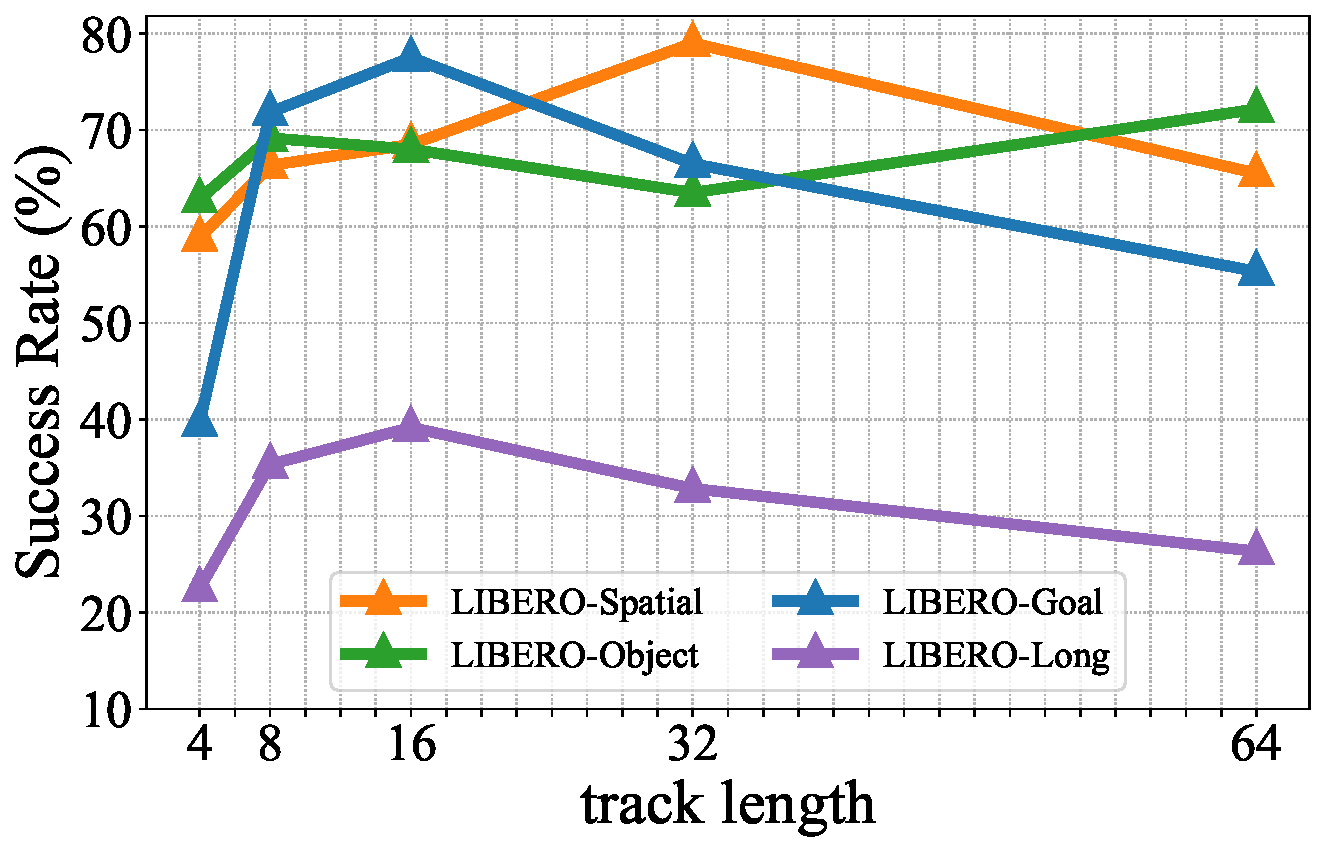
\includegraphics[width=0.9\linewidth]{fig/libero-track-length-longer.pdf}
    \caption{We plot the success rates of the policies learned with predicted trajectories of different lengths. Generally, longer trajectory length improves the performance, but the benefit tends to plateau after 16.}
    \label{fig:libero-track-len}
\end{figure}

\begin{table*}[ht]
  \centering
  \caption{Ablation study on image masking of track transformer, where ``w/o image masking" represents that we do not mask out image patches during track transformer training and ``w/ image masking" means we randomly mask 50\% patches. We can see that mask image modeling in track transformer improves the policy performance.}
  \begin{tabular}{@{}ccccc@{}}
    \toprule
    Image Mask Ratio & Spatial & Object & Goal & Long \\
    \midrule
    w/o image masking & $69.17\pm6.38$ & $65.00\pm3.89$ & $74.33\pm3.66$ & $30.83\pm11.43$ \\
    w/ image masking (default) & $68.50\pm1.78$ & $68.00\pm6.18$ & $77.83\pm0.82$ & $39.33\pm15.80$ \\
    \bottomrule
  \end{tabular}
  \label{tab:ablation-mask-ratio}
\end{table*}

\begin{table*}[ht]
  \centering
  \caption{Ablation study on the policy architecture. We explore the effect of the tracks fed into the policy in two positions:  transformer input (early fusion) and MLP head (late fusion), as illustrated in Figure~\ref{fig:track_policy}.}
  \begin{tabular}{@{}cccccc@{}}
    \toprule
    early fusion & late fusion & Spatial & Object & Goal & Long \\
    \midrule
    \CheckmarkBold & \XSolidBrush & $44.67\pm1.84$ & $56.67\pm3.09$ & $5.33\pm0.24$ & $22.33\pm4.94$ \\
    \XSolidBrush & \CheckmarkBold & $65.50\pm3.89$ &  $60.00\pm1.47$ & $72.83\pm4.73$  & $42.76\pm14.62$ \\
    \midrule
    \CheckmarkBold & \CheckmarkBold & $68.50\pm1.78$ & $68.00\pm6.18$ & $77.83\pm0.82$ & $39.33\pm15.80$ \\
    \bottomrule
  \end{tabular}
  \label{tab:arch-ablation}
\end{table*}

\noindent\textbf{Effect of track length.}
The track length of our pre-trained track transformer is 16 and we utilize all 16 points of each track by default as input for our policy.
In this experiment, we investigate the effect of track length of our policy input, by training our policy with the predicted tracks truncated into 4, 8, and 16 steps.
The results in Figure~\ref{fig:libero-track-len} demonstrate that longer tracks result in higher success rates in general, except LIBERO-Object where track length $=8$ yields the best performance. 
In particular, reducing track length leads to larger performance drops on LIBERO-Goal and LIBERO-Long.
These tasks require a comprehensive understanding of the task goal. Longer tracks provide more detailed and specific subgoals for each task, which is crucial for guiding the agent's movements and actions in subsequent stage. 
Conversely, for LIBERO-Object, which emphasizes precision operations over understanding of the task goal, a policy with a length of 16 underperforms slightly compared to the model with a length of 8. We hypothesize that the longer tracks might interfere with the learning of inverse dynamics due to noise. This also supports our approach of employing tracks both as subgoal conditions and in leveraging the nature of inverse dynamics.


\noindent\textbf{Effect of image masking in track transformer.}
When training the track transformer, we randomly mask out patches in the images and learn to reconstruct them as an auxiliary task. We conduct an ablation study by removing the image masking loss and comparing it against our standard configuration, where we randomly mask out $50\%$ of the image masks. In Table~\ref{tab:ablation-mask-ratio}, the results reveal a slight decline in policy performance when image masking is omitted, suggesting image masking can be a useful auxiliary task, except on LIBERO-Spatial. We hypothesize that the auxiliary loss encourages the model to jointly reason about different regions of an image observation. This bias may not be critical for the Libero-spatial tasks because the specific spatial location of interest is already fully specified in the language instruction (e.g., all tasks have the format of "pick up the black bowl at [some spatial location]"). 

\noindent\textbf{Effect of early and late fusion in policy architecture.}
As shown in Figure~\ref{fig:track_policy}, the predicted tracks are fed into the policy both before and after the transformer architecture within the policy, which we call early fusion and late fusion respectively. We conduct ablation studies by removing these two track inputs. The results are shown in Table~\ref{tab:arch-ablation}. We can see that removing the late fusion leads to the most significant performance drop; on LIBERO-Goal, \textit{w/ only early fusion} performs similarly to other baselines, whereas only late fusion performs marginally worse than our full method. This suggests a late fusion of the predicted tracks acts as useful subgoals that help the policy better understand the tasks in a multi-task learning setting. The subgoal prediction is more robust as it is trained on a larger video dataset.